\documentclass[11pt, A4paper,norsk]{article}
\usepackage[utf8]{inputenc}
\usepackage[T1]{fontenc}
\usepackage{babel}
\usepackage{amsmath}
\usepackage{amsfonts}
\usepackage{amsthm}
\usepackage{amssymb}
\usepackage[colorlinks]{hyperref}
\usepackage{listings}
\usepackage{color}
\usepackage{hyperref}
\usepackage{graphicx}
\usepackage{cite}
\usepackage{textcomp}
\usepackage{float}

\definecolor{dkgreen}{rgb}{0,0.6,0}
\definecolor{gray}{rgb}{0.5,0.5,0.5}
\definecolor{daynineyellow}{rgb}{1.0,0.655,0.102}
\definecolor{url}{rgb}{0.1,0.1,0.4}

\lstset{frame=tb,
	language=Python,
	aboveskip=3mm,
	belowskip=3mm,
	showstringspaces=false,
	columns=flexible,
	basicstyle={\small\ttfamily},
	numbers=none,
	numberstyle=\tiny\color{gray},
	keywordstyle=\color{blue},
	commentstyle=\color{daynineyellow},
	stringstyle=\color{dkgreen},
	breaklines=true,
	breakatwhitespace=true,
	tabsize=3
}

\lstset{inputpath="C:/Users/Torstein/Documents/UiO/Fys2140/Python programmer"}
\graphicspath{{C:/Users/Torstein/Documents/UiO/Fys2140/"Python programmer"/}}
\hypersetup{colorlinks, urlcolor=url}

\author{Torstein Solheim Ølberg}
\title{Svar på Oblig nr. 4 i Fys2140}



%\lstinputlisting{Filnavn! type kodefil}
%\includegraphics[width=12.6cm,height=8cm]{Filnavn! type png}



\begin{document}
\maketitle
	\begin{center}
\Large \textbf{Oppgaver}
	\end{center}









		\paragraph{1.}
			\subparagraph{a)}
				\begin{flushleft}
For å finne normaliseringen til funksjonen ser jeg på funksjonen ved $t = 0$, siden . kravet for at $\psi$ skal være normalisert er da at $\int_{- \infty}^{\infty} | \psi |^2 dx = 1$
				\end{flushleft}
				\begin{gather*}
\int_{- \infty}^{\infty} |\psi(x, 0)|^2 dx = 1 \\
\int_{- \infty}^{\infty} \psi(x, 0) \psi^{*}(x, 0) dx = 1 \\
\int_{- \infty}^{\infty} Ae^{- \lambda |x|} \cdot Ae^{- \lambda |x|} dx = 1 \\
\int_{- \infty}^{\infty} |A| e^{- 2 \lambda |x|} dx = 1 \\
\text{Bruker Rotmanns integral nummer 49 på side 155, bare med absolutt verdi} \\
\text{istedenfor opphøyd i andre.} \\
2 |A|^2 \int_{0}^{\infty} e^{- 2 \lambda |x|} dx = 2 |A|^2 \left[ \frac{1}{-2 \lambda} e^{- 2 \lambda |x|} \right]_{0}^{\infty} = 1 \\
|A|^2 = \left| - \lambda \left( \frac{1}{e^{\infty}} - \frac{1}{e^{0}} \right) \right| = \lambda \\
A = \sqrt{\lambda}
				\end{gather*}









			\subparagraph{b)}
				\begin{flushleft}
Forventningsverdien verdien til $x$ er gitt ved formelen under, og velger for enkelhets skylt nå også $t = 1$
				\end{flushleft}
				\begin{gather*}
\langle x \rangle = \int_{- \infty}^{\infty} \psi^{*} x \psi dx \\
\langle x \rangle = \lambda \int_{- \infty}^{\infty} x e^{- 2 \lambda |x|} dx = \lambda \int_{- \infty}^{0} x e^{- 2 \lambda |x|} dx + \lambda \int_{0}^{\infty} x e^{- 2 \lambda |x|} dx
				\end{gather*}
				\begin{flushleft}
Dette er to integral som er fullstendig like hverandre, bortsett fra at det ene er utelukkende negativt og det andre er strengt positivt, fordi integralene er over en funksjon som blir speilet om origo. Da tilsvarer det en sum av to like integraler med hvert sitt fortegn, og svare blir null.
				\end{flushleft}
				\begin{gather*}
\langle x^2 \rangle = \int_{- \infty}^{\infty} \psi^{*} x^2 \psi dx \\
\langle x \rangle = \int_{- \infty}^{0} x^2 \lambda e^{- 2 \lambda |x|} dx + \int_{0}^{\infty} x^2 \lambda e^{- 2 \lambda |x|} dx \\
\text{Dette er to integraler som er like, men speilet om y aksen, og blir derfor bare} \\
\text{to ganger et av integralene. Dette kan vi si siden integralet er strengt positivt} \\
\langle x^2 \rangle = 2 \int_{0}^{\infty} x^2 \lambda e^{- 2 \lambda x} dx \\
\text{På grunn av formelen $\int_{0}^{\infty} x^{n} e^{-ax} dx = \frac{1}{a^{n + 1}} n!$ kan vi skrive dette på formen} \\
\frac{2!}{(2 \lambda)^{3}} = \frac{1}{4 \lambda^3} \\
\text{Da får vi at}
\langle x^2 \rangle = 2 \lambda \left( \frac{1}{4 \lambda^3} \right) = \frac{1}{2 \lambda^2}
				\end{gather*}








			\subparagraph{c)}
				\begin{flushleft}
Standardavviket er kvadratroten av variansen av fordeling.
				\end{flushleft}
				\begin{gather*}
\sigma = \sqrt{\langle x^2 \rangle - \langle x \rangle^2} = \sqrt{\frac{1}{2 \lambda^{2}} - 0} = \frac{1}{\sqrt{2} \lambda}
				\end{gather*}
				\begin{figure}[H]
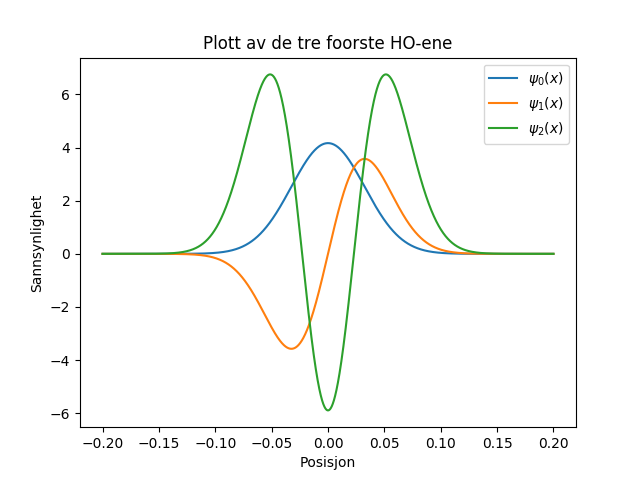
\includegraphics[width=12.6cm,height=8cm]{Figur_04.png}
\caption{Graf av psi kvadrat med $t = 0$, $\lambda = 2$ og $10000$ steg}
				\end{figure}
				\begin{flushleft}
Sannsynligheten for at vi finner partikkelen utenfor intervallet $[\langle x \rangle - \sigma, \langle x \rangle + \sigma]$ er gitt ved $\int_{- \infty}^{\langle x \rangle - \sigma} |\psi|^2 dx + \int_{\langle x \rangle + \sigma}^{\infty} |\psi|^2 dx$
				\end{flushleft}
				\begin{gather*}
P = \int_{- \infty}^{\langle x \rangle - \sigma} |\psi|^2 dx + \int_{\langle x \rangle + \sigma}^{\infty} |\psi|^2 dx \\
P = \int_{- \infty}^{- \sigma} \lambda e^{- 2 \lambda |x|} dx + \int_{\sigma}^{\infty} \lambda e^{- 2 \lambda |x|} dx \\
\text{På grunn av symetri kan dette skrives som} \\
P = 2 \int_{\sigma}^{\infty} \lambda e^{- 2 \lambda |x|} dx \\
P = 2 \lambda \left[0 - \frac{e^{- 2 \lambda \sigma}}{- 2 \lambda} \right] = e^{- \frac{2 \lambda}{\sqrt{2} \lambda}} = e^{-\sqrt{2}} = 0.24311
				\end{gather*}
				\begin{flushleft}
altså er sansynligheten ca. $24\%$ for at partikkelen blir funnet utenfor det intervallet.
				\end{flushleft}
\lstinputlisting{Oblig4_1c.py}








		\paragraph{2.}
			\subparagraph{a)}
				\begin{flushleft}
Finner $A$ ved hjelp av integralet $\int_{- \infty}^{\infty} |\psi(x)|^2 dx = 1$, og ved å sette $t = 0$.
				\end{flushleft}
				\begin{gather*}
1 = \int_{- \infty}^{\infty} |\psi(x)|^2 dx = \int_{- \infty}^{\infty} A^2 e^{- 2 a \left( \frac{mx^2}{\hbar} \right)} dx \\
1 = \int_{- \infty}^{\infty} A^2 e^{- \frac{2 a m}{\hbar} x^2} dx = A^2 \int_{- \infty}^{\infty} e^{- \frac{2 a m}{\hbar} x^2} dx \\
\text{I følge likning $(49)$ på side $155$ blir dette} \\
1 = A^2 \sqrt{\frac{\pi}{\frac{2 a m}{\hbar}}} \Rightarrow A^2 = \sqrt{\frac{2 a m}{\pi \hbar}} \Rightarrow A = \sqrt[4]{\frac{2 a m}{\pi \hbar}} = \sqrt[4]{\frac{4 a m}{h}}
				\end{gather*}










			\subparagraph{b)}
				\begin{flushleft}
Setter $\psi(x, t) = \sqrt[4]{\frac{4 a m}{h}}e^{-a \left(\frac{mx^2}{\hbar} + it\right)}$ inn i Schrödinger likningen.
				\end{flushleft}
				\begin{gather*}
i \hbar \frac{\partial \psi}{\partial t} = - \frac{\hbar^2}{2m} \frac{\partial^2 \psi}{\partial x^2} + V(x) \psi \\
i \hbar \frac{\partial}{\partial t} \left( \sqrt[4]{\frac{4 a m}{h}}e^{-a \left(\frac{mx^2}{\hbar} + it\right)} \right) = - \frac{\hbar^2}{2m} \frac{\partial^2}{\partial x^2} \left( \sqrt[4]{\frac{4 a m}{h}}e^{-a \left(\frac{mx^2}{\hbar} + it\right)} \right) + V(x) \left( \sqrt[4]{\frac{4 a m}{h}}e^{-a \left(\frac{mx^2}{\hbar} + it\right)} \right) \\
\hbar a e^{- a \left( \frac{m x^2}{\hbar} + it \right)} = - \frac{\hbar^2}{2 m} \frac{\partial}{\partial x} \left(- \frac{2 a m x}{\hbar} e^{-a \left( \frac{m x^2}{\hbar} + it \right)} \right) + V(x) e^{-a \left(\frac{mx^2}{\hbar} + it\right)} \\
\hbar a e^{- a \left( \frac{m x^2}{\hbar} + it \right)} = \hbar a \left(1 - \frac{2a mx^2}{\hbar} \right) e^{- a \left( \frac{m x^2}{\hbar} + it \right)} + V(x)e^{- a \left( \frac{m x^2}{\hbar} + it \right)} \\
0 = e^{- a \left( \frac{m x^2}{\hbar} + it \right)} \left( \hbar a - \hbar a - 2 a^2 m x^2 + V(x) \right) \\
V(x) = 2a^2 m x^2
				\end{gather*}









			\subparagraph{c)}
				\begin{gather*}
\langle x \rangle = \int_{-\infty}^{\infty} \psi^{*} x \psi dx = \int_{-\infty}^{\infty} x A^2 e^{- \frac{2 a m x^2}{\hbar}} dx \\
\langle x \rangle = \int_{- \infty}^{- 0} x A^2 e^{- \frac{2 a m x^2}{\hbar}} dx + \int_{+ 0}^{\infty} x A^2 e^{- \frac{2 a m x^2}{\hbar}} dx \\
\text{På grunn av symmetri blir disse integralene like, bare med motsatt fortegn} \\
\langle x \rangle =  \int_{0}^{\infty} x A^2 e^{- \frac{2 a m x^2}{\hbar}} dx - \int_{0}^{\infty} x A^2 e^{- \frac{2 a m x^2}{\hbar}} dx = 0
				\end{gather*}
				\begin{gather*}
\text{Finner for $x^2$} \\
\langle x^2 \rangle = \int_{-\infty}^{\infty} \psi^{*} x^2 \psi dx = \int_{-\infty}^{\infty} x^2 A^2 e^{- \frac{2 a m x^2}{\hbar}} dx \\
\langle x^2 \rangle = \int_{- \infty}^{- 0} x^2 A^2 e^{- \frac{2 a m x^2}{\hbar}} dx + \int_{+ 0}^{\infty} x^2 A^2 e^{- \frac{2 a m x^2}{\hbar}} dx \\
\text{På grunn av symmetri blir disse integralene like, og begge positive} \\
\langle x^2 \rangle = 2 \int_{0}^{\infty} x^2 A^2 e^{- \frac{2 a m x^2}{\hbar}} dx = 2 \sqrt{\frac{4 a m}{h}} \int_{0}^{\infty} x^2 e^{- \frac{2 a m}{\hbar} x^2} dx \\
\text{Bruker det bestemte integralet $(50)$ fra Rottman på side $155$} \\
\langle x^2 \rangle = \sqrt{\frac{4 a m}{h}} \left( \frac{2 a m}{\hbar} \right)^{- \frac{2 + 1}{2}} \Gamma \left( \frac{2 + 1}{2} \right) = \frac{1}{\sqrt{\pi}} \left( \frac{2 a m}{\hbar} \right)^{\frac{1}{2} - \frac{3}{2}} \Gamma \left( \frac{3}{2} \right) \\
\text{Bruker så at $\Gamma \left( \frac{3}{2} \right) = \frac{1}{2} \sqrt{\pi}$ som du finner på Wikipedia $(1)$} \\
\langle x^2 \rangle = \frac{1}{\sqrt{\pi}} \frac{\hbar}{2 a m} \frac{1}{2} \sqrt{\pi} = \frac{\hbar}{4am}
				\end{gather*}
				\begin{gather*}
\text{Finner for $p$} \\
\langle p \rangle = \int_{-\infty}^{\infty} \psi^{*} \frac{\hbar}{i} \frac{\partial}{\partial x} \psi dx = \int_{-\infty}^{\infty} A e^{- \frac{a m x^2}{\hbar}} \frac{\hbar}{i} \frac{\partial}{\partial x} A e^{- \frac{a m x^2}{\hbar}} dx \\
\langle p \rangle = \int_{-\infty}^{\infty} A e^{- \frac{a m x^2}{\hbar}} \frac{\hbar}{i} \frac{-2amx}{\hbar} A e^{- \frac{a m x^2}{\hbar}} dx \\
\langle p \rangle = \int_{-\infty}^{-0} \frac{-2amA^2}{i} xe^{- \frac{2 a m x^2}{\hbar}}  dx + \int_{0}^{\infty} \frac{-2amA^2}{i} xe^{- \frac{2 a m x^2}{\hbar}}  dx \\
\text{Dette blir også null på grunn av symetri} \\
				\end{gather*}
				\begin{gather*}
\text{Finner så forventet verdi for $p^2$} \\
\langle p^2 \rangle = \int_{-\infty}^{\infty} \psi^{*} \left( \frac{\hbar}{i} \frac{\partial}{\partial x} \right)^2 \psi dx = \int_{-\infty}^{\infty} A^2 \left(- \hbar^2\right) e^{- \frac{a m x^2}{\hbar}} \left(- \frac{2am}{\hbar} \left( \frac{- 2amx^2}{\hbar} + 1 \right) e^{-\frac{amx^2}{\hbar}} \right) dx \\
\langle p^2 \rangle = \frac{2am\hbar}{\sqrt{\pi}} \sqrt{\frac{2am}{\hbar}} \int_{-\infty}^{\infty} \left( \frac{- 2amx^2}{\hbar} + 1 \right) e^{- \frac{2 a m x^2}{\hbar}} dx \\
\langle p^2 \rangle = \frac{2am\hbar}{\sqrt{\pi}} \sqrt{\frac{2am}{\hbar}} \left( \int_{-\infty}^{\infty} \frac{- 2amx^2}{\hbar} e^{- \frac{2 a m x^2}{\hbar}} dx + \int_{-\infty}^{\infty} e^{- \frac{2 a m x^2}{\hbar}} dx \right) \\
\text{Kan skrive integralene om på grunn av symetri} \\
\langle p^2 \rangle = \frac{2am\hbar}{\sqrt{\pi}} \sqrt{\frac{2am}{\hbar}} \left( \left(- \frac{2am}{\hbar} \right) 2 \int_{0}^{\infty} x^2e^{- \frac{2amx^2}{\hbar}} dx + 2 \int_{0}^{\infty} e^{- \frac{2amx^2}{\hbar}} dx \right) \\
\text{Bruker integralet fra oppgave når vi finner $\langle x^2 \rangle$} \\
\langle p^2 \rangle = \frac{2am\hbar}{\sqrt{\pi}} \sqrt{\frac{2am}{\hbar}} \left( \left(- \frac{2am}{\hbar} \right) \left( \frac{2am}{\hbar} \right)^{-\frac{3}{2}} \frac{1}{2} \sqrt{\pi} + 2 \frac{1}{2} \left( \frac{2am}{\hbar} \right)^{-\frac{1}{2}} \sqrt{\pi} \right) \\
\langle p^2 \rangle = - \frac{2am\hbar}{\sqrt{\pi}} \sqrt{\frac{2am}{\hbar}} \left(\left( \frac{2am}{\hbar} \right)^{-\frac{1}{2}} \frac{1}{2} \sqrt{\pi} - \frac{2am}{\hbar} ^{-\frac{1}{2}} \sqrt{\pi} \right) \\
\langle p^2 \rangle = - \frac{2am\hbar}{\sqrt{\pi}} \left( \frac{\sqrt{\pi}}{2} \left( \frac{2am}{\hbar} \right)^{\frac{1 + 2 - 3}{2}} - \sqrt{\pi} \right) \\
\langle p^2 \rangle = - am\hbar + 2am\hbar = am\hbar
				\end{gather*}










			\subparagraph{d)}
				\begin{gather*}
\sigma_x^2 = \langle x^2 \rangle - \langle x \rangle^2 \Rightarrow \sigma_x = \sqrt{\frac{\hbar}{4am}} \\
\sigma_p^2 = \langle p^2 \rangle - \langle p \rangle^2 \Rightarrow \sigma_p = \sqrt{am\hbar} \\
\sigma_x \sigma_p = \sqrt{\frac{\hbar}{4am}} \sqrt{am\hbar} = \frac{\hbar}{2} \\
\frac{\hbar}{2} \geq \frac{\hbar}{2} \\
\text{Som er akkurat det vi trenger.}
				\end{gather*}











		\paragraph{3.}
			\begin{gather*}
\text{Legger til en konstant $V_0$ til den potensielle energien} \\
i \hbar \frac{\partial \psi}{\partial t} = - \frac{\hbar}{2m} \frac{\partial^2 \psi}{\partial x^2} + \left( V + V_0 \right) \psi \\
\text{Det vi ønsker å ende opp med er: $i \hbar \frac{\partial \psi'}{\partial t} = - \frac{\hbar}{2m} \frac{\partial^2 \psi'}{\partial x^2} + V(x) \psi'$} \\
\text{Der $\psi' = \psi e^{-\frac{iV_0t}{\hbar}}$. Derfor ganger vi med eksponenten} \\
i \hbar \frac{\partial \psi}{\partial t} e^{-\frac{iV_0t}{\hbar}} = - \frac{\hbar}{2m} \frac{\partial^2 \psi}{\partial x^2} e^{-\frac{iV_0t}{\hbar}} + \left( V + V_0 \right) \psi e^{-\frac{iV_0t}{\hbar}} \\
i \hbar \frac{\partial \psi}{\partial t} e^{-\frac{iV_0t}{\hbar}} = - \frac{\hbar}{2m} \frac{\partial^2 \psi'}{\partial x^2} + \left( V + V_0 \right) \psi' \\
i \hbar \frac{\partial \psi}{\partial t} e^{-\frac{iV_0t}{\hbar}} - V_0 \psi' = - \frac{\hbar}{2m} \frac{\partial^2 \psi'}{\partial x^2} + V \psi' \\
i \hbar \left( \frac{\partial \psi}{\partial t} e^{-\frac{iV_0t}{\hbar}} - \frac{iV_0}{\hbar} \psi e^{-\frac{iV_0t}{\hbar}} \right) = - \frac{\hbar}{2m} \frac{\partial^2 \psi'}{\partial x^2} + V \psi' \\
\text{Hvis vi bruker kjerneregelen på det som er inni parantesen så ser vi at dette blir lik} \\
i \hbar \frac{\partial \psi'}{\partial t} = - \frac{\hbar}{2m} \frac{\partial^2 \psi'}{\partial x^2} + V \psi' \\
\text{Siden alle forventningsverdier er tidsuavhengige vil ikke en ekstra tidsavhengig} \\
\text{faktor ha noe som helst å si.}
			\end{gather*}







	\begin{center}
\Large \textbf{Bibliografi}
	\end{center}
		\begin{flushleft}
$(1)$ \url{https://en.wikipedia.org/wiki/Gamma_function}
		\end{flushleft}
\end{document}